\documentclass[10pt,a4paper]{article}
\usepackage[utf8]{inputenc}
\usepackage[ngerman]{babel}
\usepackage[T1]{fontenc}
\usepackage{amsmath}
\usepackage{amsfonts}
\usepackage{amssymb}
\usepackage{graphicx}
\usepackage{lmodern}
\usepackage{physics}
\usepackage[left=2cm,right=1cm,top=2cm,bottom=1.5cm,twoside]{geometry}
\usepackage{siunitx}
\usepackage{fancyhdr}
\usepackage{enumerate}
\usepackage{mhchem}
\usepackage{mathtools}
\usepackage{graphicx}
\graphicspath{./Figures}
\usepackage{float}
\usepackage{xcolor}
\usepackage{mdframed}
\usepackage{csquotes}
\usepackage{trfsigns}
\usepackage{capt-of}
\usepackage{listings}
\setlength{\headheight}{23pt}
\setlength{\headsep}{10pt}
\setlength{\marginparwidth}{0pt}
% \setlength{\parindent}{0pt}
\usepackage{enumitem}

\sisetup{locale=DE}
\sisetup{per-mode = symbol-or-fraction}
\sisetup{separate-uncertainty=true}
\DeclareSIUnit\year{a}
\DeclareSIUnit\clight{c}
\mdfdefinestyle{exercise}{
	backgroundcolor=black!10,roundcorner=8pt,hidealllines=true,nobreak
}

\definecolor{codegreen}{rgb}{0,0.6,0}
\definecolor{codegray}{rgb}{0.5,0.5,0.5}
\definecolor{codepurple}{rgb}{0.58,0,0.82}
\definecolor{backcolour}{rgb}{0.95,0.95,0.95}
\renewcommand{\lstlistingname}{Code}% Listing -> Algorithm
\renewcommand{\lstlistlistingname}{List of \lstlistingname s}% List of Listings -> List of Algorithms
\lstdefinestyle{mystyle}{
    backgroundcolor=\color{backcolour},
    commentstyle=\color{codegreen},
    keywordstyle=\color{magenta},
    numberstyle=\tiny\color{codegray},
    stringstyle=\color{codepurple},
    basicstyle=\ttfamily\footnotesize,
    breakatwhitespace=false,
    breaklines=true,
    captionpos=b,
    keepspaces=true,
    numbers=left,
    numbersep=3pt,
    showspaces=false,
    showstringspaces=false,
    showtabs=false,
    tabsize=3
}
\lstset{style=mystyle}


\begin{document}
\twocolumn
\pagestyle{fancy}
\lhead{Formelsammlung}
\rhead{Maximilian Binninger}
\cfoot{\vspace{-20pt}\thepage}

\section{Grundlagen}
Linearisierung um Arbeitspunkt:
\begin{align*}
	x_{a}(t)=x_{a,AP}+\Delta x_{a}(t) \approx x_{a,AP}+\sum\left(\frac{\partial f}
	{\partial x_{e,Ap}} \cdot \Delta x_{e}(t)\right)
\end{align*}
Kräftegleichungen:
\begin{mdframed}[style=exercise]
	Federkraft: $F_F$ = $k_F \cdot x$\\
	Dampfkraft: $F_D$ = $k_D \cdot v$ = $k_D \cdot \dot{x}$\\
	Trägheitskraft: $F_{Tr}$ = $m\cdot a$ = $m\cdot \ddot{x}$\\
	Erdanziehungskraft: $F_G$ = $m\cdot g$
\end{mdframed}
Moment Gleichungen:
\begin{mdframed}[style=exercise]
	Widerstandsmoment: $M_w$ = $k_D \cdot \omega$\\
	Trägheitsmoment: $M_{TR}$ = J$\cdot \dot{\omega}$
\end{mdframed}
Spannungsgleichung:
\begin{mdframed}[style=exercise]
	\[
		U = L\cdot \frac{di}{dt}+i\cdot R+\frac{1}{C} \cdot \int i
	\]
\end{mdframed}
Für kleine Winkel $\alpha$ gilt: sin($\alpha$) = $\alpha$\\
Rotation in Flüssigkeit:
\[
	M=M_{\texttt{Träg}}+M_{\texttt{Brems}}=J \cdot \dot{\omega} +k_{\texttt{Flüssigkeit}} \cdot \omega
\]\\
Partialbruchzerlegung (siehe Papula s.157ff)\\
\\
Anfangswertsatz: $x(t \rightarrow +0)=\lim _{s \rightarrow \infty} s \cdot X(s)$\\
Endwertsatz: $x(t \rightarrow \infty)=\lim _{s \rightarrow 0} s \cdot X(s)$
\section{Systemtechnik}
\subsection{Modellbildung}
Hinweise zum aufstellen der Differentialgleichung eines Systems:
\begin{mdframed}[style=exercise]
	\begin{enumerate}
		\item Bestimmung der Ein- und Ausgangsgrößen
		\item Suche nach dem beschreibenden Gleichgewicht
		\item In der Gleichung dürfen nur Konstanten, sowie die Ein- und
		      Ausgangsgrößen in beliebiger Ableitung vorkommen
		\item Andere Variablen müssen durch erlaubte Größen ersetzt werden\\
		      \footnotesize
		      (Dazu können i.a. physikalische Gleichungen benutzt werden)
	\end{enumerate}
\end{mdframed}

\subsection{Signalflussplan/Blockschaltbild}
Erzeugung des Signalflussplans aus der Zugehörigen DGL.
\begin{mdframed}[style=exercise]
	\begin{enumerate}
		\item für technische Realisierung gilt: m < n;

		\item DGL. nach höchster Ableitung der Ausgangsgröße auflösen

		\item höchste Ableitung der Ausgangsgröße geht auf den Eingang des ersten Integrators\\
		      \footnotesize
		      (Laplace-Trans ersetzt das Integrieren mit einer Division mit „s“)
	\end{enumerate}
\end{mdframed}
\begin{center}
	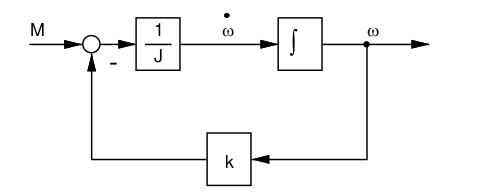
\includegraphics[width=0.96\columnwidth]{Figures/Signalflussplan12.png}
\end{center}

Erzeugung des Signalflussplans eines Systems mit der DGL.:

\begin{align*}
	  & a_{n} \overset{(n)}{x}_{a}+\ldots+a_{2} \ddot{x}_{a}+a_{1} \dot{x}_{a}+a_{0} x_{a} \\
	= & b_{n} \overset{(n)}{x}_{e}+\ldots+b_{2} \ddot{x}+b_{1} \dot{x}_{e}+b_{0} x_{e}
\end{align*}

Signalflussplan kann allgemein gezeichnet werden: (nötig, falls eine Ableitung von $x_e$ existiert)

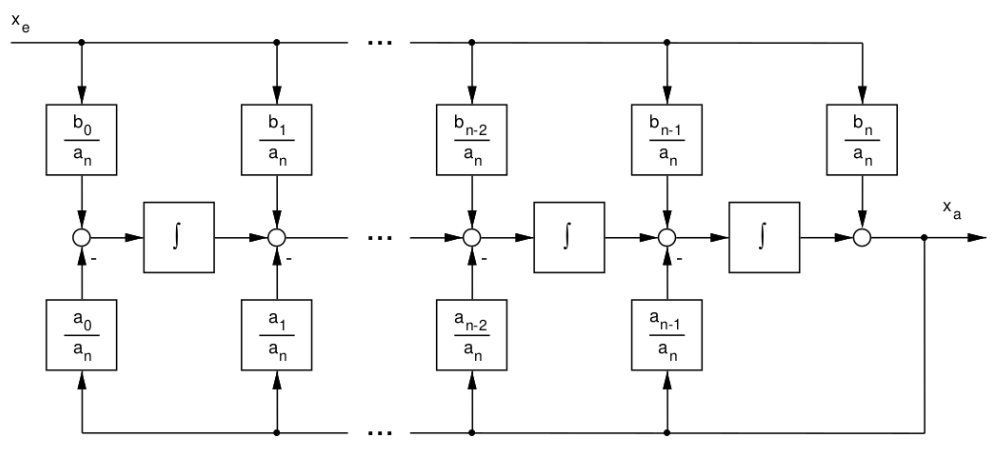
\includegraphics[width=0.9\columnwidth]{Figures/SFmitDGL.png}

\subsection{Stabilität}
\begin{mdframed}[style=exercise]
	BIBO-Stabilität (Bounded Input/ Bounded Output-> begrenzt):\\
	ein dynamisches System ist stabil, wenn gilt:\\
	für ein begrenztes $x_e$ gibt es immer ein begrenztes $x_a$
\end{mdframed}

\subsection{Ortskurven und Frequenzkennlinien}

Ortskurvendarstellung:
\begin{center}
	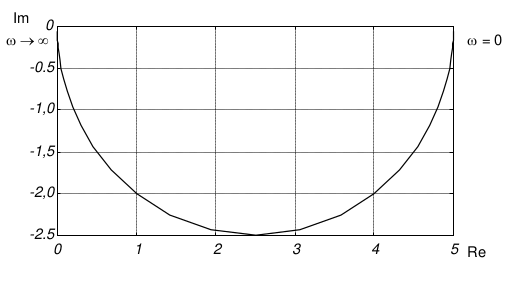
\includegraphics[width=0.96\columnwidth]{Figures/Ortskurve.png}
\end{center}
\begin{mdframed}[style=exercise]
	Für wachsendes $\omega$ werden die komplexen Werte F(j$\omega$) in die
	komplexe F-Ebene eingetragen und zur Ortskurve verbunden.\\ Jeder
	Ortskurvenpunkt kann jetzt als Zeiger gedeutet werden.
\end{mdframed}

\newpage
Bodediagramm Darstellung:
\begin{center}
	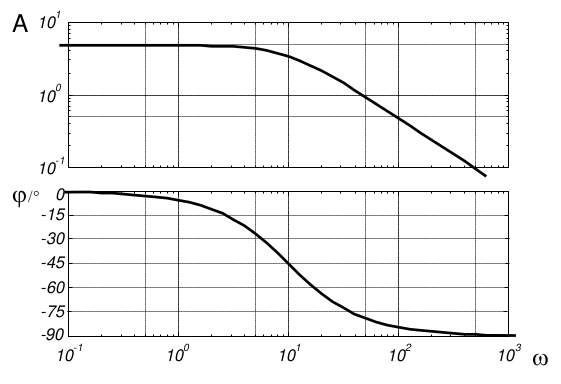
\includegraphics[width=0.96\columnwidth]{Figures/Bodediagramm.png}
\end{center}
\begin{mdframed}[style=exercise]
	Der Amplitudengang A($\omega$) wird in doppelt logarithmischer Darstellung
	aufgetragen,\\ der Phasengang y($\omega$)) halblogarithmisch. Gemeinsame
	Abszisse ist $\omega$.

	Bei diesem Beispiel (PT1-Glied) ist deutlich der\\ Tiefpass-Charakter zu
	erkennen.

	Verkettete Funktionen im Bodediagramm resultieren als Produkt der
	Einzelübertragungsfunktionen.

	D.h. Verstärkung wird multipliziert und Phasenverschiebung addiert.\\ Das
	heißt: Sowohl Phasengang (halblogarithmische Darstellung) und Amplitudengang
	(logarithmische Darstellung) werden graphisch addiert!
\end{mdframed}

\subsection{$\mathbf{F(s)}$ in Pol- und Nullstellenform}
\begin{mdframed}[style=exercise]
	Zähler- und Nennerpolynom von F(s) besitzt Nullstellen. Diese sind von
	$a_v$ und $b_u$ abhängig.\\
	Nullstellen des Zählers sind Nullstellen von F(s)\\
	Nullstellen des Nenners sind Polstellen von F(s)\\
	Wenn Pole $s_pv$ und Nullstellen $s_nu$ bekannt, kann man F(s) mit dem
	Faktor Q in faktorisierter Form darstellen.
\end{mdframed}

\[
	F(s)=Q \cdot \frac{\prod_{\mu=1}^{m}\left(s-s_{N \mu}\right)}{\prod_{v=1}^{n}\left(s-s_{P V}\right)}
	\qquad \texttt{mit } Q = \frac{b_m}{a_n}
\]

\begin{mdframed}[style=exercise]
	Die Stabilität von $F(s)$ kann anhand der Lage der Pole $s_pv$ in der s-Ebene
	beurteilt werden.\\ $F(s)$ ist stabil, wenn alle Pole $s_pv$ in der linken
	s-Halbebene liegen.\\ Instabile Pole in der Rechten Halbebene lassen sich
	nicht durch Reihenschaltung mit entsprechender Nullstelle kompensieren!
\end{mdframed}
\begin{mdframed}[style=exercise]
	Bedeutung Polstelle:

	Pole bewirken ein zeitverzögertes Verhalten. Je weiter links sie sich befinden,
	desto schneller ist der Einschwingvorgang.

	$\Rightarrow$ Wenn Pole deutlich weiter links liegen als andere andere, kann man sie ohne
	großen Fehler vernachlässigen.
\end{mdframed}
\begin{mdframed}[style=exercise]
	Bedeutung Nullstelle:\\
	NS bewirken ein differenzierendes Verhalten (Beschleunigung des Systems)
	Einfluss weit links in der s-Ebene kann häufig vernachlässigt werden.

\end{mdframed}

\subsection{Signalflussplan Algebra}
\begin{itemize}[leftmargin=*]
	\item Kettenstruktur:
	      \begin{center}
		      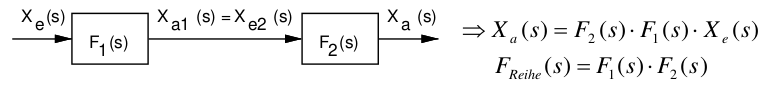
\includegraphics[width=0.96\columnwidth]{Figures/Kettenstruktur.png}
	      \end{center}

	\item Parallelstruktur:
	      \begin{center}
		      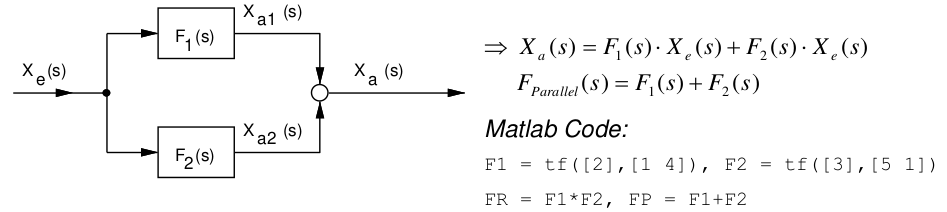
\includegraphics[width=0.96\columnwidth]{Figures/Parallelstruktur.png}
	      \end{center}

	\item Kreisstruktur:
	      \begin{center}
		      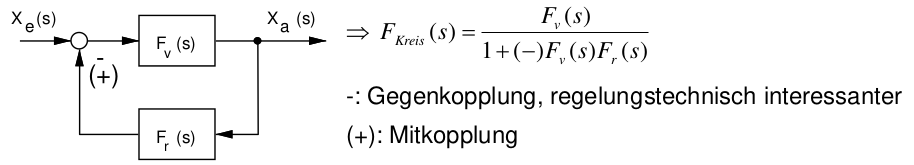
\includegraphics[width=0.96\columnwidth]{Figures/Kreisstruktur.png}
	      \end{center}

	\item Verschieben einer Additionsstelle:
	      \begin{center}
		      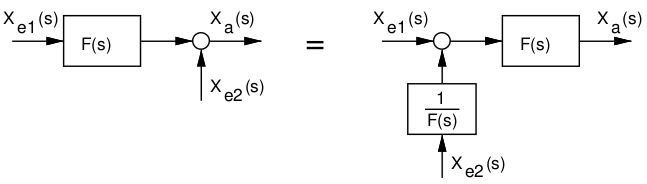
\includegraphics[width=0.9\columnwidth]{Figures/Verschiebung einer Additionsstelel.png}
	      \end{center}

	\item Verschieben einer Verzweigung:
	      \begin{center}
		      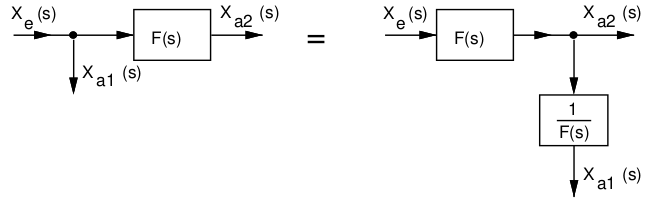
\includegraphics[width=0.9\columnwidth]{Figures/Verschiebung einer Verzweigung.png}
	      \end{center}
\end{itemize}

\section{Zusammenwirken mehrerer Systeme}
\subsection{Regelkreis}
\begin{mdframed}[style=exercise,frametitle=Anforderungen:]
	\begin{itemize}[leftmargin=*]
		\item Stabilität: Regelkreis muss stabiles Verhalten zeigen (gilt
		      auch für instabile Systeme)
		\item Gutes Führungsverhalten: Die Differenz zw. Sollwert w(t) und
		      Istwert x(t) muss schnell klein werden.
		\item Gutes Störverhalten: Einfluss von Störgrößen soll vermindert
		      werden.
	\end{itemize}
\end{mdframed}

Grundstruktur des einschleifigen Regelkreises:

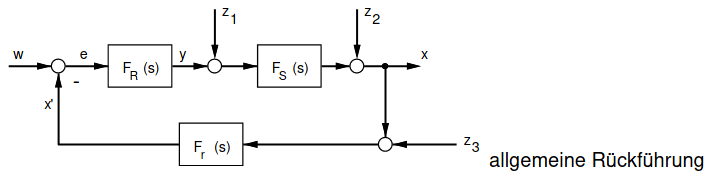
\includegraphics[width=0.9\columnwidth]{Figures/einschleifiger Regelkreis.png}

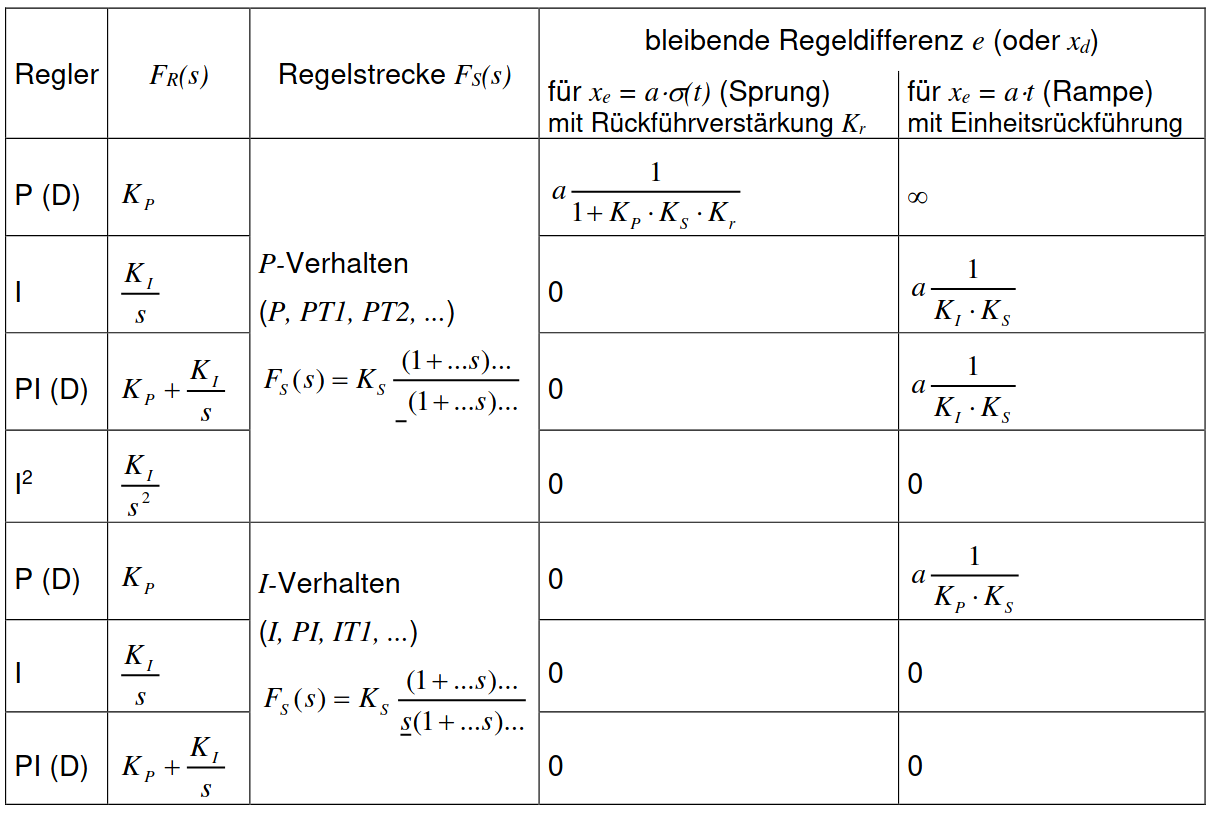
\includegraphics[width=0.94\columnwidth]{Figures/Reglerauswahl.png}


\subsection{Wurzelortskurven (WOK)-Verfahren}
\begin{mdframed}[style=exercise]
	Reglerfunktion $F_R$ in Reglerverstärkung und Reglerdynamik aufspalten:
	$F_R =K \cdot F_R ' $
\end{mdframed}

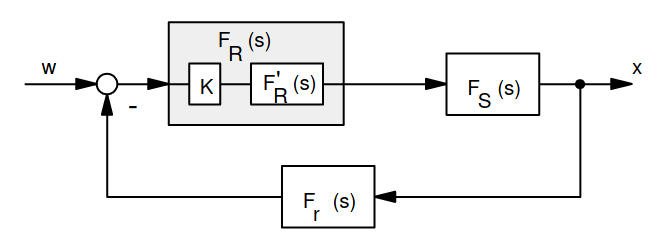
\includegraphics[width=0.94\columnwidth]{Figures/WOKkreis.png}
\[
	\Rightarrow F_w (s)= \dfrac {F_R \cdot F_S} {1+F_R \cdot F_S \cdot F_r}
\]

\begin{mdframed}[style=exercise]
	Dabei ist $F_o = F_R \cdot F_S \cdot F_r$ die Übertragungsfunktion des
	offenen Regelkreises. $F_o$ kann auch in faktorisierter Form angegeben
	werden:
\end{mdframed}

\begin{align*}
	F_w (s) & = F_R (s) \cdot F_S (s) \cdot F_r (s)
	\\ & =K \cdot F_R '(s) \cdot F_S (s) \cdot F_r (s)
	\\ & =K \cdot Q \cdot \frac{\prod_{u=1}^{m}\left(s-s_{\text {Nou
			}}\right)}{\prod_{v=1}^{n}\left(s-s_{\text {pov }}\right)}
\end{align*}

Für eine Polstele, muss der Nenner von $F_w (s)$ Null werden:
\[
	\dfrac{F_R (s) \cdot F_S (s)}{1+F_o (s)} \Rightarrow 1+F_o (s) \stackrel{!}{=}0
\]

Daraus folgt:
\begin{align*}
	 & \Rightarrow 1+ K \cdot Q \cdot \frac{\prod_{M=1}^{m}\left(s-s_{\text {Nou }}\right)}{\prod_{v=1}^{n}\left(s-s_{\text {por }}\right)}         \\
	 & \Rightarrow \frac{\prod_{v=1}^{n}\left(s-s_{\text {pov }}\right)}{\prod_{u=1}^{m}\left(s-s_{\text {Nou }}\right)} \stackrel{!}{=} -K \cdot Q
\end{align*}

Entspricht: $\frac{\texttt{Multiplikation aller PS zum gesuchten Punkt}}
	{\texttt{Multiplikation aller NS zum gesuchten Punkt}}$

\subsection{Konstruktion der WOK}
\begin{mdframed}[style=exercise]
	\begin{enumerate}[leftmargin=*]
		\item Alle n Äste der WOK beginnen mit K=0 in den n Polen $s_pov$ des offenen Regelkreises.
		\item m Äste der WOK enden für K $\rightarrow \pm \infty$
		\item n -m Äste der WOK enden für K $\rightarrow \pm \infty$ im Unendlichen
		\item Die n-m ins Unendliche strebende Äste der WOK haben Asymptoten,die\\
		      a) im Wurzelschwerpunkt
		      \[S_{w}=\frac{\sum_{v=1}^{n} s_{pov}-\sum_{u=1}^{m} s_{_{Nop}}}{n-m}\]
		      beginnen und die dabei\\
		      b) mit der reellen Achse die Winkel\\
		      $\varphi_{k}=\frac{(2 k-1) \cdot 180^{\circ}}{n-m}$ für KQ > 0 bzw.\\
		      mit k = 1,2,3,\dots,n-m
		\item Die Punkte der WOk liegen entweder auf der reelen Achse, oder symmetrisch zur reelen Achse
		\item Ein Punkt s auf der reellen Achse ist dann ein Punkt der WOK, wenn sich bei KQ > 0 (KQ<0)
		      rechts von ihm eine ungerade (gerade) Anzahl von Polen $s_{pov}$ und (+) Nullstellen $s_{Nov}$ befindet.
	\end{enumerate}

	Achtung: WOK ist nicht anwendbar, wenn es sich um nicht rationale
	Übertragungsfunktionen handelt.\\ (z.B. Regelkreis mit Totzeitverhalten!)
\end{mdframed}

\subsection{Nyquist Kriterium}
\begin{center}
	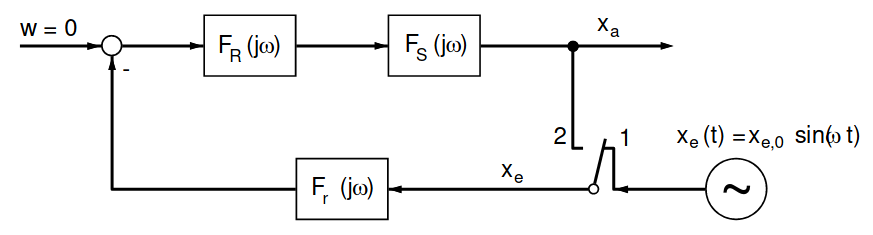
\includegraphics[width=.45\textwidth]{Figures/Nyquist.png}
\end{center}
Frequenzgangfunktion des offenen Regelkreises:
\[
	F_o (j\omega) = F_r (j\omega) \cdot F_R (j\omega) \cdot F_S (j\omega)
\]

Ausgangssignal:
\begin{align*}
	x_a(t) & =-F_r (j\omega) \cdot F_R (j\omega) \cdot F_S (j\omega) \cdot
	x_{e0}sin(\omega t)                                                    \\
	       & = -F_0 (j\omega) \cdot x_e (t)
\end{align*}

Regler und seine Parameter werden so gewählt,\\ dass $\omega = \omega_{krit}$ gilt:
\[
	-F_0 (j\omega_{krit})=1 \text{ oder } F_0 (j\omega_{krit})=-1 \texttt{ (Schwingbedingung)}
\]

\begin{mdframed}[style=exercise]
	Die Schwingbedingung ist erfüllt, wenn die Ortskurve von $F_1 (j\omega)$
	durch den kritischen Punkt ($P_{krit} = -2+j0$) der komplexen $F_0$-Ebene
	geht.

	An diesem Punkt kann man $\omega_{krit}$ ablesen (damit kann der Regelkreis
	Dauerschwingungen ausführen).

	Für größere $\omega$ ist das System instabil, für kleinere stabil.
\end{mdframed}

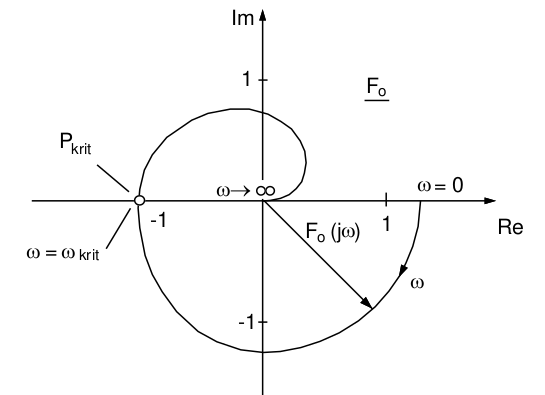
\includegraphics[width=0.94\columnwidth]{Figures/Nyquistwkrit.png}

\begin{mdframed}[style=exercise]
	Falls F(s) des offenen Kreises keine Pole in der rechten Halbebene hat und
	nur max. 2 im Ursprung der s-Ebene, ist der Regelkreis stabil, wenn der
	kritische Punkt von $\omega$ immer links von s = -1 + 0j liegt.

	\footnotesize
	(gilt immer wenn der offene Kreis stabil ist)
\end{mdframed}

Zur Auswertung des Nyquist-Kriteriums im Bode Diagramm, spaltet man die Ortskurve nach Betrag
A = |$F_0 (jw)$ und Phase $\varphi$ = $F_0(jw)$

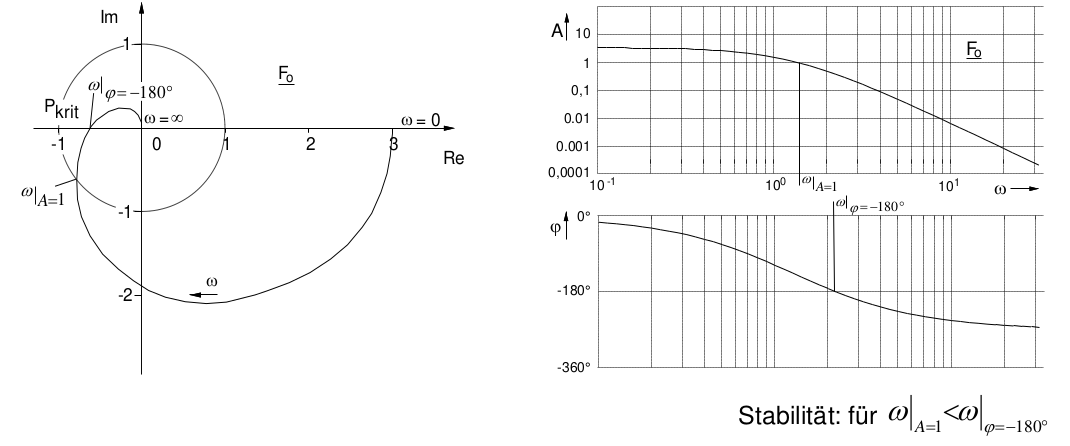
\includegraphics[width=0.94\columnwidth]{Figures/Nyquist_Bode.png}

Falls die Bedingung nicht funktioniert, wird die allgemeine Formulierung verwendet:

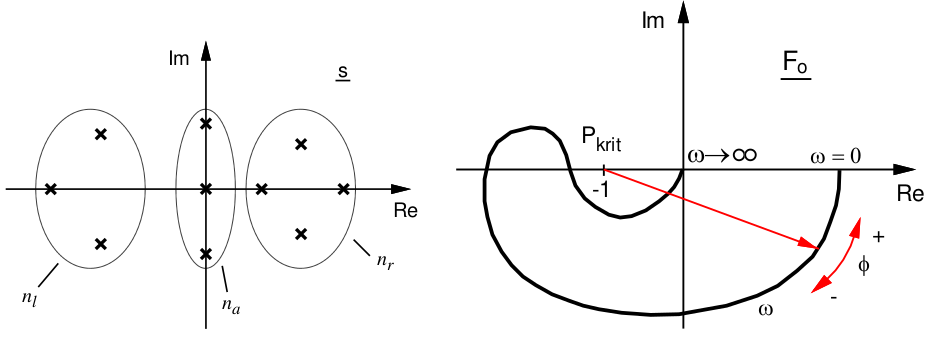
\includegraphics[width=0.94\columnwidth]{Figures/Allgemein_Nyquist.png}

\begin{mdframed}[style=exercise]
	Der geschlossene Regelkreis ist stabil, wenn der Fahrstrahl von $P_{krit}$ = -1 +j0
	zu $F_0 (jw)$ für wachsendes $\omega$ von +0 bis +$\infty$ eine Winkeländerung
	$^{\omega=+\infty}_{\omega=+0} \Delta \phi _{soll} = n_r \cdot$ 180° $+n_a \cdot$ 90°
	erfährt.\\
	$n_r$: Anzahl der Pole rechts der imaginären Achse\\
	$n_a$: Anzahl der Pole auf der imaginären Achse
\end{mdframed}

\subsubsection{Phasenrad/Phasenreserve:}

\begin{itemize}[leftmargin=*]
	\item[] Aus Bodediagramm ablesen: Bei Verstärkung von 1
	\item[] Winkeln von -180° nach oben rechnen
	\item befriedigendes Verhalten bei Störungen gilt: $\varphi _R \geq 30\circ$
	\item gutes Verhalten (überschwingungsarm) gilt: $\varphi _R \approx  60\circ$
	\item gutes Verhalten (überschwingungsfrei) gilt: $\varphi _R \geq 80^\circ$
\end{itemize}

\subsection{Einstellregler Ziegler/Nichols}
\subsubsection{Maßnahmen zur Verbesserung des Regelkreisverhaltens und Erweiterungen der Regelkreisstruktur}

\centering
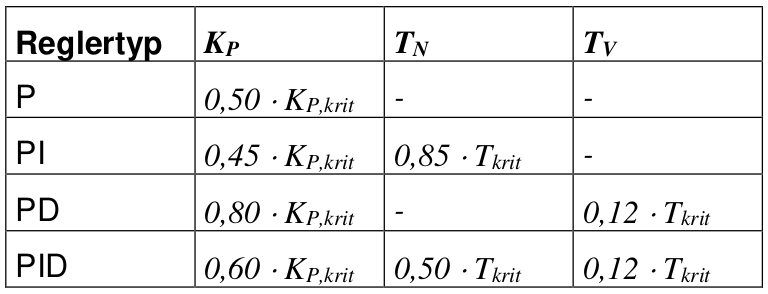
\includegraphics[width=0.9\columnwidth]{Figures/ZieglerNich.png}\\

\raggedright
\begin{mdframed}[style=exercise, frametitle=Störgrößenaufschaltung:]
	Falls Angriffsort einer Störgröße bekannt,kann man wie im Bild kompensieren.\\
	Vorteil: einfacher Regler Entwurf, deutlich schnellere Ausregelung.
\end{mdframed}

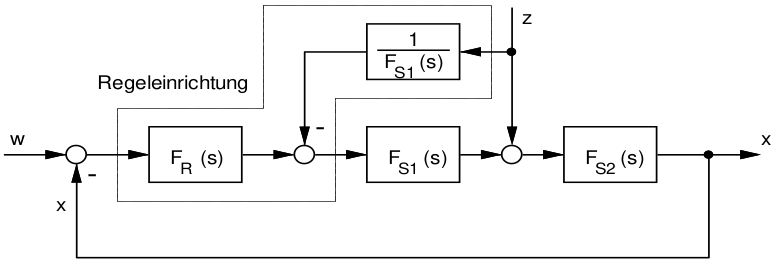
\includegraphics[width=0.9\columnwidth]{Figures/Stoergoesenschaltung.png}


\begin{mdframed}[style=exercise, frametitle=Vorsteuerung:]
	Geeignet, falls kein Kompromiss für gutes Stör und Folgeverhalten.\\
	Regler ist auf gutes Störverhalten ausgelegt. Mit $F_{Rv}$ wird ein schnelles Folgen
	auf Führungssignale w(t) erreicht.
\end{mdframed}

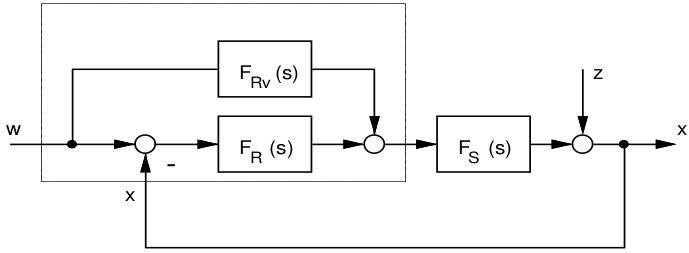
\includegraphics[width=0.9\columnwidth]{Figures/Vorsteuerung.png}


\begin{mdframed}[style=exercise, frametitle=Kaskadenregelung:]
	Ineinander geschachtelte Regelkreise (innere Regelkreise „schneller“). „Innere“
	Störungen können bereits innen ausgeregelt werden. Können von Innen nach Außen in Betrieb genommen werden.
\end{mdframed}

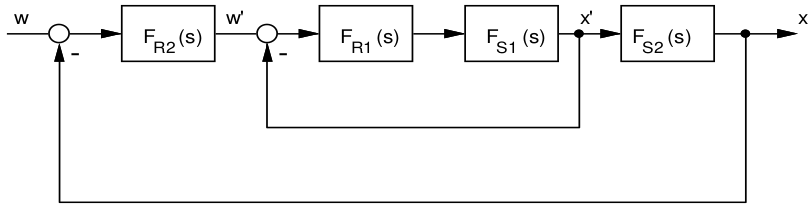
\includegraphics[width=0.9\columnwidth]{Figures/Kaskadenregelung.png}

\newpage
\section{Digitale Regler}
\subsection{Allgemeines}
\subsubsection{z-Transformation}

Wert der bei t = k $\cdot T_A$ ausgegeben wird, wird bei t = (k-1) $\cdot T_A$
eingelesen. (Verzögerung um einen Abtastschritt):

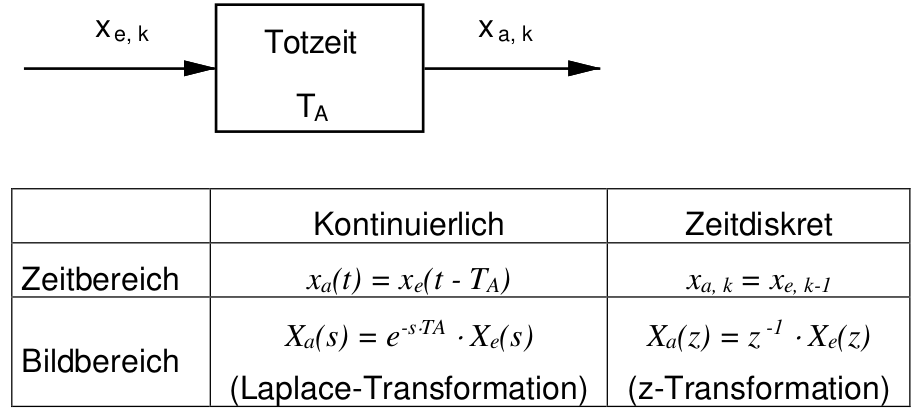
\includegraphics[width=0.9\columnwidth]{Figures/zTrans.png}

Bei der z-Transformation entspricht $e^{-s \cdot TA}$ der
Laplace-Transformation dem Ausdruck $z^{-1}$. Bzw. z $\hat{=}$ $e^{s \cdot
			TA}$\\ Transformation vom s-Bereich in den z-Bereich:
\[
	s \ \hat{=}\  e^{s \cdot TA}
\]

Vorwärts-Differenzen-quotient
\[
	s \ \hat{=} \ \frac{z-1}{T_A}
\]

$\Rightarrow$ Der digitale Regler kann folgend berechnet werden:
\[
	F(z) = F(z)|_{s= \frac {z-1}{T_A}}
\]

Tustinsche Formel
\[
	s \ \hat{=} \ \frac{2}{T_A} \cdot \frac{z-1}{z+1}
\]

Rückwärts-Differenzen-quotient

\section{Systembeschreibung im Zustandsraum}
\subsection{Allgemein (Mehrgrößensystem MIMO) }
\begin{mdframed}[style=exercise]
	\vspace{-1em}
	\begin{align*}
		\dot{\Vec{x}}(t) & = A\vec{x}(t) + B\vec{u}(t) \quad x(0) = x_{0} \\
		\vec{y}(t)       & = C\vec{x}(t) + D\vec{u}(t)
	\end{align*}
\end{mdframed}

\begin{center}
	\includegraphics[width=0.96\columnwidth]{Figures/Signalflussplan.png}
	\captionof{figure}{Signalflussplan}
\end{center}

\begin{mdframed}[style=exercise]
	\begin{align*}
		\dot{x}_{1} & = 0\cdot x_{1} +0\cdot x_{2} +0\cdot x_{3} +1\cdot u_{1}+0\cdot u_{2}        \\
		\dot{x}_{2} & = K\cdot x_{1} +0\cdot x_{2} +0\cdot x_{3} +0\cdot u_{1}+0\cdot u_{2}        \\
		\dot{x}_{3} & = 0\cdot x_{1} +0\cdot x_{2} +0\cdot x_{3} +H\cdot J\cdot u_{1}+J\cdot u_{2} \\
		\dot{y}_{1} & = 0\cdot x_{1} +1+x_{2} +0\cdot x_{3} +0\cdot u_{1}+0\cdot u_{2}             \\
		\dot{y}_{2} & = 0\cdot x_{1} +0\cdot x_{2} +l\cdot x_{3} +0\cdot u_{1}+0\cdot u_{2}        \\
	\end{align*}
\end{mdframed}

\begin{mdframed}[style=exercise]
	\[
		\ A = \begin{bmatrix}
			0 & 0 & 0 \\
			K & 0 & 0 \\
			0 & 0 & 0
		\end{bmatrix}
		C = \begin{bmatrix}
			0 & 1 & 0 \\
			0 & 0 & l \\
		\end{bmatrix}\]
	\[B = \begin{bmatrix}
			1         & 0 \\
			0         & 0 \\
			H\cdot{}J & J
		\end{bmatrix} \
		D = \begin{bmatrix}
			0 & 0 \\
			0 & 0
		\end{bmatrix}
	\]

	Eigenwerte einer Matrix bestimmen (z.B. A):
    \[
        \operatorname{det}(A - sI) \overset{!}{=} 0
    \]
\end{mdframed}

\subsubsection{Polfestlegung durch vollständige Zustandsrückführung}

\centering
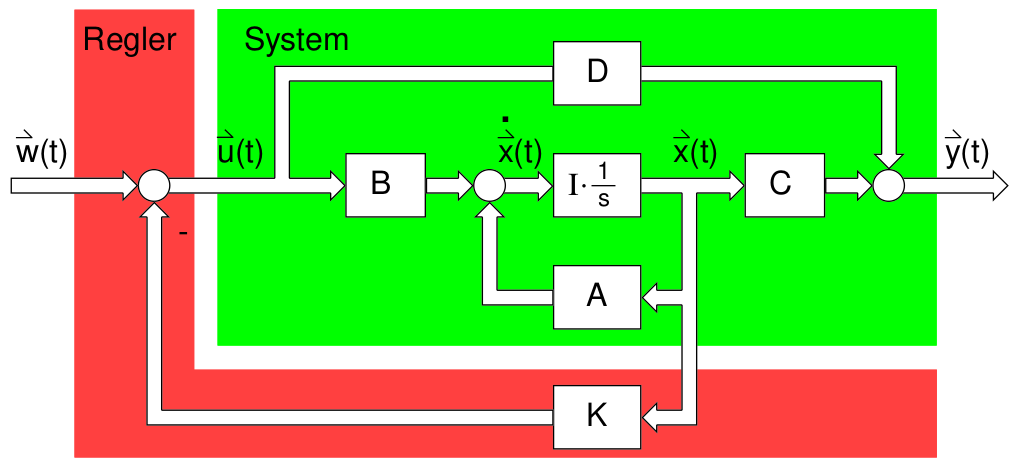
\includegraphics[width=0.8\columnwidth]{Figures/Polfestlegung.png}

\raggedright
Durch die freie Wahl von K können alle n Pole des Systems beliebig platziert
werden.

Rückführungsverstärkung: von jedem X einen Pfad zur größten Ableitung
mit Verstärkung K zeichnen. Über neue Matrix und deren determinante kann dann
die Reglerverstärkung bestimmt werden.

\begin{mdframed}
\[
	A = \begin{bmatrix}
		B(a-K)
    \end{bmatrix}
\]
\begin{center}
    \footnotesize a ist vorfaktor der $\vec{x}(t)$, siehe oben.
\end{center}
\end{mdframed}

dann mit der Determinante der Matrix A: K bestimmen mit den gegebenen Polen

\subsection{Programmtechnische Umsetzung}
Zähler und Nenner der z-Übertragungsfunktion durch die höchste Potenz teilen

\begin{lstlisting}[language=Matlab]
  while(1)
  {
      waitinterrupt(T_A); //Abtastzeit warten
      xout2 = xout1;
      xout1 = xout;
      xin2 = xin1;
      xin1 = xin;
      input(xin);
      xout = k*xout2 - j*xin1 + o*xout1;
      output(xa);
  }
\end{lstlisting}

\end{document}
